\subsection{\label{subsec:FZV1}Frage 1}
\textbf{\textit{Wie kann aus der interferometrischen Autokorrelationsfunktion die Pulsdauer 
bestimmt werden? Nehmen Sie einen Gaußpuls an.}}\\
$\rightarrow$In einem Michelson-Interferometer kann der kurze Eingangspuls 
in zwei identische Pulse aufgeteilt werden, die dann nach einer zeitlichen Verzögerung
$\Delta \tau=\frac{\Delta{s}}{c}$ wieder kombiniert werden. Mit Hilfe eines, im Vergleich 
zum Puls, langsam messenden Detektors wird die gemittelte Energie der überlagernden 
Puls-Felder aufgezeichnet. Die Form lässt sich mathematisch beschreiben \cite{UltraFast}
\begin{align}
    \langle P_{\text{out}}\rangle &= \frac{1}{2}\Gamma_{a}(0) + \frac{1}{2}|\Gamma_{a}(\Delta \tau)|\cos(\omega_{0}\Delta\tau + \Phi(\Delta\tau)) \\
    \Gamma_{a}(\Delta \tau) &= \int_{-\infty}^{\infty}\,a^{*}(t)a(t+\Delta \tau) dt,
\end{align}  
wobei $a(t)$ das elektrische Feld des Pulses beschreibt. \\
Im Allgemeinen lässt sich die Pulsdauer aus dieser Messung nicht bestimmen, was jedoch nicht 
auf einen Gaußpuls zutrifft. Die Faltung zweier solcher Signale liefert erneut einen Gaußpuls mit einer
veränderten Breite, die direkt aus der Einhüllenden der Energieoszillationen 
($\propto \Gamma_{a}(\Delta \tau)$) abgelesen werden kann. 
Es gilt 
\begin{align}
    \Gamma_{a}(\Delta \tau) &= \frac{1}{2\pi\sigma}\int_{-\infty}^{\infty}\,e^{-\frac{1}{2}(\frac{t}{\sigma})^{2}}
    e^{-\frac{1}{2}(\frac{t+\Delta \tau}{\sigma})^{2}} dt \\
    &= \frac{1}{2\sqrt{\pi}\sigma}e^{-\frac{1}{2}(\frac{\Delta \tau}{\sqrt{2}\sigma})^{2}}.
\end{align}
Hieraus ist erkennbar, dass die Pulsdauer $\Delta t$ des eingehenden Gaußpulses über die Halbwertsbreite der 
Einhüllenden zu $\Delta t = \Delta \tau_{\text{FWHM}}/\sqrt{2}$ bestimmt werden kann. \\

\textbf{\textit{Bestimmen Sie aus dem optischen Spektrum des Lasers aus Abb.~3.1 die spektrale
Breite $\Delta \nu$.}}\\
$\rightarrow$Zuerst muss das Maß für die spektrale Breite ermittelt werden. 
In der Ultrakurzzeit-Physik wird die Bandbreite typischerweise als die volle Breite bei 
der Hälfte des Maximalwerts des positiven Frequenzanteils des Leistungsspektrums gemessen und wird, 
gemäß der englischen Übersetzung (Full Width at Half Maximum), 
als $\Delta \nu_{\text{FWHM}}$ bezeichnet \cite{UltraFast}. \\
Da das Intensitätsspektrum (direkt proportional zum Leistungsspektrum) als Funktion der 
Wellenlänge $\lambda$ angegeben ist, lesen wir zunächst die Wellenlängen ab, bei der die Intensität auf 
die Hälfte abfällt. Das Spektrum ist in Abb.~\ref{fig:spektrum} dargestellt.
\begin{figure}[h!]
    \centering
    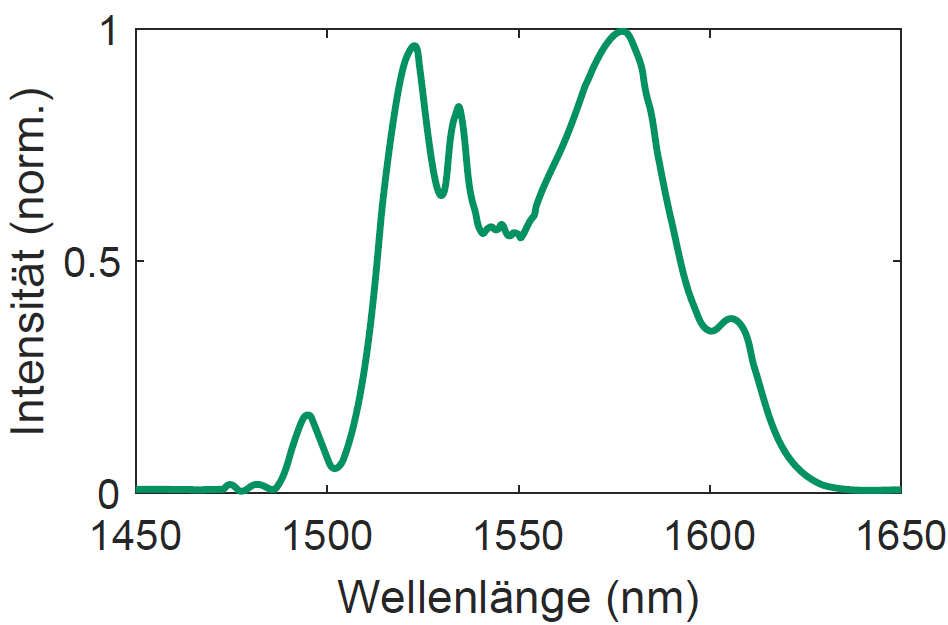
\includegraphics[width=0.4\textwidth]{LaserSpekt.png}
    \caption{\label{fig:spektrum}Das Intensitätsspektrum des im ersten Versuchsteil verwendeten Lasers
    als Funktion der Wellenlänge. Die Graphik wurde aus der Versuchsanleitung \cite{Anleitung} entnommen.}
\end{figure}\FloatBarrier 
Wir erhalten inklusive eines abgeschätzten Ablesefehlers 
\begin{equation}
    \lambda_{1} = (1515\pm 3)\,\si{nm} \hspace{0.5cm} \text{und} \hspace{0.5cm} \lambda_{2} = (1592\pm3 )\,\si{nm},
\end{equation}
woraus wir die spektrale Breite wie folgt berechnen
\begin{align}
    \Delta \nu &= c (\lambda_{1}^{-1} - \lambda_{2}^{-1}) \\
    \Rightarrow \Aboxed{\Delta \nu &= (9,6 \pm 0,5)\,\si{THz}}. \label{eq:spektrale}
\end{align} \newpage

\textbf{\textit{Wie lautet der theoretische Wert des Zeit-Bandbreiten-Produkts für
einen ideal gaußförmigen Puls?}}\\
$\rightarrow$Das Zeit-Bandbreiten-Produkt lässt sich über die Pulsdauer $\Delta t$, sowie die 
oben definierte spektrale Breite bestimmen. 
Eine Alternative Beschreibungsmethode über die root-mean-square (rms) Puls- und Bandbreite 
ist in Ref.~\cite{UltraFast} dargestellt. \\
Betrachtet man das Feld eines idealen Gaußpulses 
$a(t)=\frac{1}{\sqrt{2\pi \tau^{2}}}e^{-\frac{1}{2}(\frac{t}{\tau})^{2}}$, erhält man für die 
Breite (bezogen auf die Leistung $P(t)=|a(t)|^{2}$) des Gaußpulses $\Delta t_{FWHM} = \tau\,2\sqrt{\ln(2)}$. 
Der relevante Teil des Leistungsspektrums ergibt sich aus der Fouriertransformierten des Gaußpulses zu 
$|E(\omega)|^{2} = \frac{1}{4}\left\vert\frac{1}{2\pi}e^{-\frac{1}{2}\tau^{2}(\omega-\omega_{0})^{2}}\right\vert^{2}$, woraus 
eine spektrale Breite von $\Delta \omega_{FWHM} = \frac{1}{\tau}\,2\sqrt{\ln(2)}$ folgt.
Insgesamt ergibt sich für das Zeit-Bandbreiten-Produkt eines ideal gaußförmigen Pulses
\begin{equation}
    \fbox{$\Delta t_{\text{FWHM}}\Delta \nu_{\text{FWHM}} = \frac{2\ln(2)}{\pi} \approx 0,441$}.
\end{equation}
Ein sehr kurzer Puls besteht folglich aus vielen Frequenzkomponenten, was einer große spektralen 
Breite entspricht. \\

\textbf{\textit{Wozu wird eine Kompensationsplatte in Abb.~2.4 benötigt?}}\\
$\rightarrow$Durch den Einsatz dieser Kompensationsplatte wird gewährleistet, dass beide Lichtwege 
identisch sind. Der Strahl, der zuerst transmittiert wird, legt im Vergleich zum zuerst 
reflektierten Strahl das dreifache der Strecke durch das Glas-Substrat des Strahlteilers zurück. 
Um eine klare Interferenz sicherzustellen, ist es erforderlich, im anderen Strahlengang eine 
Kompensationsplatte einzufügen, die die Strahldispersion ausgleicht \cite{OpticsHand}.

